\documentclass[iop]{emulateapj}
\usepackage{graphicx,pdfpages,array,amsmath}

\newcommand{\fmod}{\mbox{$f_{mod,i}$}}
\newcommand{\chisq}{\mbox{$\chi^2$}}
\newcommand{\fobs}{\mbox{$f_{obs,i}$}}
\newcommand{\vij}{\mbox{$V_{ij}$}}
\newcommand{\bj}{\mbox{$B_{j}$}}
\newcommand{\sigi}{\mbox{$\sigma_{i}$}}

\begin{document}
\title{Eclipse Mapping Code}
\author{Woody Austin}

\begin{abstract}
pass
\end{abstract}
\maketitle

% INTRO
%The program is designed to model exhibit variability 
%in their light curve due to starspots rotating in and out of view on the surface of the star as
%well as features

\section{Set-up and Terminology \label{terminology}}
The eclipse mapping program described in this paper derives a model for the relative surface
brightness of a transiting planet host star when given a single band, high cadence light curve
of the target as an input.  Each run of the program produces a static surface map.
However, by applying the code to a series of short segments of the 
light curve, we are able to derive a model for the time evolution of the star's surface brightness.  

The stellar rotation period, $P_{rot}$, is an input parameter into the program 
along with the orbital and physical properties of the planet, including the
planet radius relative to the host star, $r_{p}$, the orbital period, $P_{orb}$, etc.   **OTHER INPUTS Need defining?**
The star is assumed to be rotating as a uniform solid body.  In addition, we require the spin-axis of the star   
to be aligned with the orbital axis of the planet and the planet to be on a circular orbit.  
%These criteria are both met for our test object, Kepler-17 \cite{}.  }

In order to efficiently {\bf describe the details of our program}, the geometry
of the problem must be defined and some basic terminology must be established.
We divide the stellar surface into a series of large {\it regions}, as shown in Figure~\ref{fig:CoRoT}.  
While describing our program in this paper, the regions along the line of transit will be called {\it boxes}; 
the total longitudinal regions will be called {\it longitudes};
and the longitudinal regions with the box areas subtracted will be referred to as {\it stripes}.
When talked about as an ensemble or when the distinction is unimportant, these regions will be referred to as just that - {\it regions}. 

++++STOPPED HERE++++

Typically, 

%causing the regions to rotate in and out of view over time.  


The surface brightness, $b_j$, of
each region is held constant 

longitudinal stripes. Additionally, we add a set of boxes that lie along the path of the eclipsing planet

\begin{figure}[h]
	\centering
	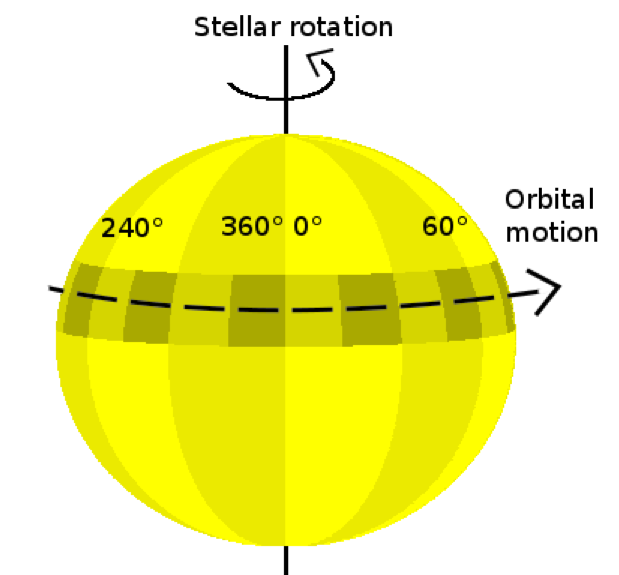
\includegraphics[width=.5\textwidth]{modelGeometry.png}
	\caption{CoRoT brightness map.}
	\label{CoRoT}
\end{figure}


Our program calculates the model flux at each time step, by summing over the surface of the visible sphere according to:

\begin{equation}
	\fmod = \sum_j V_{i,j}b_j, 
\end{equation}

where $b_j$ is the brightness per unit area for region $j$ and $V_{i,j}$ is the {\it visibility} of that region at time, $i$.


This model flux has two parts: a visibility and a brightness value. The amoeba determines the brightness values while the visibility values are pre-defined. Both of these apply to a set of $j$ regions. 
The planet will occlude only the boxes and will do so only during a transit. The longitudes' brightness values are defined as:

\begin{equation}
Z_j = \frac{S_j - \frac{c}{q} \sum_{j=1}^{q}B_j}{1- c}
\end{equation}

Where $q$ is the ratio of $n_{boxes}$ to $n_{stripes}$ and $c$ is the ratio of the total eclipsed area to the non-eclipsed area. $c$ can be calculated by the same set of integrals that will be used for the visibilities.

If the Amoeba algorithm is given the set of boxes and stripes, they will be able to vary to offset each other creating a "zebra" pattern in the brightness map.  The longitude values create parameter independence by warping the chi-squared space so that such a case is less likely to become a local minimum. The Amoeba algorithm takes the set of box brightness guesses and longitude brightness guesses as inputs. During each call of the chi-squared algorithm the stripe values are calculated from the longitudes and boxes. The boxes and the stripes are then used to calculate the model flux.

\vspace{9mm}
\section{The transiting planet model \label{transit_model}}
To actually model the starspot features within the transit portions of the light curve, a reasonable understanding of the visibility profile of a transit for any given system is required. The visibility of the transits is determined by the portion of the star that the planet occludes during transit and some limb darkening effects. As discussed earlier, the planet will only transit along the boxes contained within the latitudes at $\pm r_p$ from the impact parameter, b. 
 
The first step in determining the visibility occluded by a planet at a given time step involves simple geometry which will then be extended to the ten cases contained in Table~\ref{cases}. The simplifying approximation that each of the boxes is a cartesian rectangle when it is projected onto the surface of the star is made. Although this is not entirely accurate, it is a good approximation because when it overestimates a portion of the box, it must also underestimate a similar but not necessarily equal portion of the box.

The simplest case in which the planet is entirely contained within a box is:
\begin{equation}
	A_{occluded} = \pi r_p^2
\end{equation}

The planet can also be partially contained in a box in many ways, shown in Table~\ref{cases}. The sliver of the planet that is not within the box will be calculated and then extended to take care of all of the various cases. To do this, the area of a sector of a circle is found and then the triangle that is formed within it is subtracted. The sector is the combination of the light blue and yellow regions in Figure~\ref{eclipse}.
\begin{figure}[h]
	\centering
	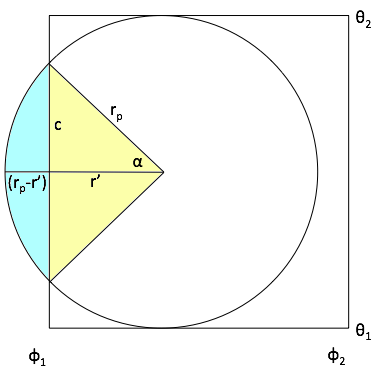
\includegraphics[width=.5\textwidth]{figure.png}
	\caption{Geometry of eclipse path visibility.}
	\label{eclipse}
\end{figure}

\begin{equation}
	A_{sector} = \frac{r_p \alpha^2}{2}
\end{equation}

where:

\begin{equation}
	\alpha = 2 \cos^{-1}\left(\frac{r^{\prime}}{r_p}\right)
\end{equation}

The area of the triangle is $cr^{\prime}$. $c$ is one half the length of the chord in the figure. $c$ can be found with the Pythagorean theorem. Knowing this, the area of the triangle becomes: 

\begin{equation}
	A_{triangle} = r^{\prime}\sqrt{r_p^2 - {r^{\prime}}^2}
\end{equation}

Finally, the area of the segment that indicates the part of the planet just over the border of the box is:

\begin{equation}
	A_{seg} = r_p^2 \cos^{-1}\left(\frac{r^{\prime}}{r_p}\right) - r^{\prime} \sqrt{r_p^2 - {r^{\prime}}^2}
\end{equation}

Using $A_{seg} $ and Table~\ref{cases}, a believable box-car transit model is produced. However, limb darkening must also be included in order to give a better approximation to the actual shape of a real transit. Limb darkening is introduced in the visibility rather than in the model flux calculation. This is okay because $\fmod = V_{i,j} b{j}$. If limb-darkening were calculated during every flux calculation of every chi-squared call during the Amoeba algorithm run, it would require much more operational complexity in the code. However, limb-darkening can be calculated before the many chi-squared calls via the Amoeba algorithm and and avoid this.  The geometric analysis of the transit and limb darkening is continued in the next section.

\begin{table}
	\caption{Subcases for planetary eclipse visibility}
	\label{cases}
	\begin{center}
	\renewcommand{\arraystretch}{1.2}
		\begin{tabular}{| m{.04\textwidth} | m{.24\textwidth} | m{.15\textwidth} |} %c means center justify, l left, r right
			\hline
			\textbf{Case}    & \textbf{Description} & \textbf{Area covered by planet in box}\\ %Separate with &, lines with \\
			\hline%horizontal line
			I      &   Planet is completely out of the box to the right                                                                      & 0                                                           \\ \hline
			II     &   Planet is completely out of the box to the left                                                                         & 0                                                           \\ \hline
			III    &   Planet is completely contained in the box                                                                              & $\pi r_p^2$                                         \\ \hline
			IV    &   Planet is partially off the right side of the box. Center is inside of the box                       & $\pi r_p^2 - A_{seg,l}$                     \\ \hline
			V     &   Planet is partially off the right side of the box. Center is outside of the box                     & $A_{seg}$                                          \\ \hline
			VI    &   Planet is partially off the left side of the box. Center is inside of the box                          & $\pi r_p^2 - A_{seg,r}$                     \\ \hline
			VII   &   Planet is partially off the left side of the box. Center is outside of the box                        & $A_{seg}$                                          \\ \hline
			VIII  &   Planet is partially off both sides of the box. Center is inside of the box                            & $\pi r_p^2 - A_{seg,r} - A_{seg,l}$ \\ \hline
			IX    &   Planet is partially off the right side of the box. Center is outside of the box to the left & $A_{seg,l1} - A_{seg,l2}$                \\ \hline
			X     &   Planet is partially off the left side of the box. Center is outside of the box to the right    & $A_{seg,r1} - A_{seg,r2}$               \\ \hline
		\end{tabular}
	\end{center}
\end{table}

\section{Limb Darkening}
To actually calculate the limb-darkening, a quadratic limb-darkening law is used.
\begin{equation}
   \frac{I(\psi)}{I(0)} = 1 - c_1 (1 - \mu) - c_2 (1 - \mu)^2
\end{equation}
Here, $\mu$ is the cosine of the angle between the line of sight and the normal at the point at which you are trying to calculate the limb darkening. Because stars are so distant, this can be approximated as $\hat{x} = R^* \sin{\theta}\cos{\phi}$, but $R^{*}$ is defined as 1.0 throughout all calculations.

To complete the limb darkening model, the average value in one of the regions is calculated at every timestep. This is done analytically from the integral:

\begin{equation}
\begin{split}
    \frac{1}{V_{i,j}} \int_{\phi_1}^{\phi_2} & \int_{\theta_1}^{\theta_2}  (1 - c_1 (1 - \sin{\theta}\cos{\phi}) \\ &- c_2 (1 - \sin{\theta}\cos{\phi})^2) \sin{\theta}\cos{\phi}\,\mathrm{d}\theta \, \mathrm{d}\phi
\end{split}
\end{equation}

This works well for limb-darkening determination in each region, but care must be taken when calculating limb darkening for the eclipse. Rather than calculating equations of limb darkening for the eclipse directly as in Mandol \& Agol 2000, the ratio of the limb-darkened eclipsed region to the non-limb-darkened eclipsed region is used. If the number of regions in eclipse is not high enough, a boxy limb-darkening approximation to the transit path is produced using this scheme. This happens because the planet is moving too quickly relative to the surface of the star given the in-transit binning cadence. To fix this, the ratio of the limb-darkened to non-limb-darkened regions is calculated for multiple sub-regions. This gives a finer grain approximation to the real value.

\section{Visibility Calculations of Regions \label{vis}}
Recall that in order to calculate \fmod, the visibility of each region at a given time step is required. These visibilities are calculated by finding the projected surface area of a sphere for a given set of angles. The basic integral is the spherical surface integral dotted with the unit vector, $\hat{x}$, along the line-of-sight:

\begin{equation}
	V_{i,j} = \int_{\phi_1}^{\phi_2} \int_{\theta_1}^{\theta_2} \sin^2{\theta}\cos{\phi}\,\mathrm{d}\theta \, \mathrm{d}\phi
\end{equation}

\begin{figure}[h]
	\centering
	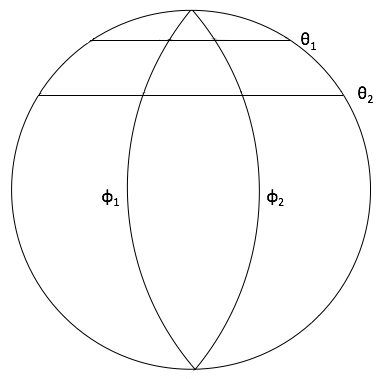
\includegraphics[width=.5\textwidth]{angles.png}
	\caption{Angles.}
	\label{angles}
\end{figure}

Where $\phi_1$, $\phi_2$, $\theta_1$, and $\theta_2$ are shown in Figure~\ref{angles}. For all types of visibilities, $\phi_1$ and $\phi_2$ are set by the number of stripes or boxes defined at the start of the program. The $\theta$ limits, however, will be different depending on region type.
The $\theta$ limits for the boxes are set by the impact parameter and the radius of the planet. The limits will be equal to $(b \pm R_p) + \frac{\pi}{2}$. The addition of $\frac{\pi}{2}$ is necessary when the bottom of the star is defined as latitude 0. For the visibility of a longitude, $\theta$ will range from 0 to $\pi$. The visibility of a stripe is calculated (in the chi-squared routine) by subtracting the sum of the box visibilities in a given longitude range from the longitude in the same range.

\section{Model Flux}
%Note: This section will be moved out of its current location
The flux of the star at any given time $i$ is given by $\fmod = \sum{V_{i,j} b_{j}}$. Each region on the star has some visibility value $V_{i,j}$ that varies with time. These visibility values are all governed by the amount of projected area that is seen by the observer over time and can be calculated via an analytical integral. Finding the brightness values, $b_j$, is the goal of the program. For a given set of data the brightness values cannot change using our technique. To remedy this, each month (or quarter) of data is divided into smaller intervals called \{it windows}. By moving the start and end times of the windows by small amounts, information about the evolution of starspots can be inferred. Previous estimates on the timescale of starspot evolution report that it occurs on the order of 10-30 days. This works well with the model described here. The model does a better job of fitting smaller sections of data than larger ones. 

The set of brightness values is optimized by minimizing the chi-squared:
\begin{equation}
	\chi^2 = \sum \frac{(\fmod - \fobs)^2}{\sigma_i^2}
\end{equation}

The Amoeba Algorithm is used to do the actual minimization. The algorithm runs quickly and will always converge given any set of inputs. The largest downside (of most optimization algorithms) is that it cannot distinguish between local and absolute minima.



\end{document}
